\documentclass[a4paper,10pt]{article}
\usepackage{fullpage}
\usepackage{amsfonts}
\usepackage[utf8]{inputenc}
\usepackage[english]{babel}
\usepackage{amsmath}
\usepackage{indentfirst}
\usepackage{graphicx}

\begin{document}
\begin{center}
Project report on\\
\vspace{0.5cm}
{{\Large \sc Artificial Intelligence Playing the Ricochet Robots Board Game}}\\
\vspace{0.5cm} for 02180 Introduction to Artificial Intelligence
\end{center}
\rule{\textwidth}{0.5pt}
\begin{description}
\item\begin{tabular}{rll}
    \textbf{Contributors:}& Jannis Haberhausen &(s186398)\\ & Jack Reinhardt &(s186182)\\ & Kilian Speiser &(s181993)\\ & Jacob Miller &(s186093) \\
\end{tabular}
\end{description}
\rule{\textwidth}{1pt}

\tableofcontents
\thispagestyle{empty}
\newpage
\section{Game Background}
\subsection{Game Rules}
\textit{Ricochet Robots} is a competitive game first published in Germany in 1999. In the original game four different colored robots are placed on a 16 by 16 board. The objective of the game is to reach a target that is placed somewhere on the board each round. The targets have different colors matching the colors of the four robots. A red target has to be reached by the red robot, a blue target by the blue robot and so on. The challenge of the game comes from the allowed movements of the robots. All robots can move in four directions: up, down, left and right, however once a robot is moved it will only stop when it hits a wall or another robot. The outer edges of the board, the four middle squares as well as additional squares on the board are blocked on up to two sides by walls. In order to reach the target often robots of other colors need to be used as 'walls'.
\begin{figure}[!htb]
\center{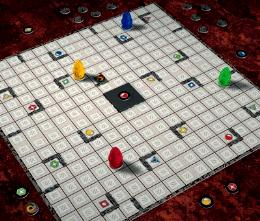
\includegraphics[width=6cm]{figures/originalgame.jpg}}
\caption{The original boardgame 'Ricochet Robots'}
\label{fig:originalgame}
\end{figure}
\subsection{Changes in the Implementation}
In the original game the board consists of four quaters printed on both sides that can be put together such that 96 unique board setups are possible. In a later version of the game there are eight quaters resulting in 1536 possible board configurations. For the assignment only one, randomly chosen, board configuration from the original game has been implemented.
\par
In order to run tests on the AIs an additional 6 by 6 board has been implemented. The game rules are exactly the same, only some squares have walls on three sides. That is because of the reduced space on the small board.
% Game rules, in particular if you choose a game not on the list above or if you make
% simplifications to the game. Make this part as short as possible. If you have simplified
% the rules, explain why and explain what it would take to make AI for the full game.

% What kind of game is it? Relevant questions are e.g.: Single- or multi-player? Competitive
% or cooperative? Zero-sum? Is it a turn-taking game? Perfect or imperfect information
% (full or partial observability)? Deterministic or stochastic? And what does this imply for
% the kind of algorithms that apply to the game?


\section{Game Representation}


\section{State Space and Complexity}
\label{sec:stateSpace}
The state space and branching factor of Ricochet Robots is large, making the task of reaching the target non-trivial for both humans and AI search algorithms.
The board consists of a sixteen-by-sixteen grid with walls placed in predetermined positions.  With four robots that can be moved anywhere on the board (other
than on top of another robot), this leaves a total of $(16*16)(16*16-1)(16*16-2)(16*16-3) = 4,195,023,360$ board configurations for a single wall setup and
target placement.  Depending on the board setup, some states may not be reachable, but the state space still remains large. Each robot can move in any of the
four directions on the board until it reaches a wall or another robot in its path.  Assuming that each robot has an obstruction in one of the four directions
decreases the possible moves for each robot to three, giving the search algorithm a branching factor of $4*3 = 12$.  This assumption will be true in most cases since
the robot must be stopped by an obstruction before moving in a different direction. \\

The large state space and branching factor makes the problem of reaching the goal state difficult for traditional AI search algorithms with limited memory and time.
In order to simplify the game and drastically reduce the size of the state space and the branching factor, we implemented Ricochet Robots in a way that allows the
user to choose the size of the board (16x16 or 6x6) as well as the number of robots. In general, the size of the state space can be approximated by $(w*h)^n$ and
the branching factor can be approximated by $n*3$, where w is the board width, h is the board height and n is the number of robots.  This reduced implementation of Ricochet Robots allowed us to play and test our AI algorithms without surpassing our memory and time limitations.


\section{Search Algorithms and Results}


  \subsection{Recursive Depth-Limited Search}


  \subsection{Informed Search: Breadth First Search}
  As already mentioned
  
  The team decided to develop a informed breadth first search to guarantee finding always the goal state by using as few moves as possible. However, this leads as mentioned in \ref{sec:stateSpace} this leads to a tree with up to $16^n$ knots.  
  \begin{itemize}
  	\item Difficulty of setting the limit to a certain level
  \end{itemize}


  \subsection{A* Search}


  \subsection{Custom Search Algorithm}


\section{Conclusion}



\end{document}
